\documentclass[12pt,a4paper]{article}%

\usepackage[utf8]{inputenc}%
\usepackage[T1]{fontenc}%
\usepackage{lmodern}%
\usepackage{amsmath, amssymb}%
\usepackage{graphicx}%
\usepackage{caption}%
\usepackage{subcaption}%
\usepackage{booktabs}%
\usepackage{geometry}%
\usepackage{natbib}%
\usepackage{setspace}%
\usepackage{hyperref}%

\geometry{left=3cm, right=2cm, top=2cm, bottom=2cm}%
\onehalfspacing%

\begin{document}
\section{Illustrative Application of the Input-Output Model}

Following the formal derivation of the environmentally extended input-output (EEIO) model, this section presents an illustrative application of the framework to household carbon footprint estimation. The aim is to operationalize the Leontief-based formulation:
\[
\mathbf{E} = \mathbf{C} (\mathbf{I}-\mathbf{A})^{-1} \mathbf{F}
\]
where $\mathbf{F}$ denotes the final demand vector, here represented by annual household consumption expenditure by category; ${(\mathbf{I}-\mathbf{A})}^{-1}$ is the Leontief inverse, capturing direct and indirect production requirements to satisfy $\mathbf{F}$; $\mathbf{C}$ is the vector of direct emission intensities (kg CO$_{2}$e per unit output).

In this illustration, pre-calculated environmentally extended emission intensities (kg CO$_{2}$e per euro spent) are applied to household consumption data for France, Spain, and Germany for 2021. These intensities represent the aggregated effect of $\mathbf{C} {(\mathbf{I}-\mathbf{A})}^{-1}$ and are derived from the EXIOBASE multi-regional input-output (MRIO) model, as accessed via Climatiq.io. The method aligns with the tier-3 comprehensive accounting approach discussed in Matthews et al.~(2008), Long et al.~(2019), and Sheng et al.~(2024).

\subsection{Data and Methodology}

Household final consumption expenditure data were obtained from Eurostat and supplementary sources, converted to euros at the 2021 average exchange rate (1 USD = 0.85 EUR). Table~\ref{tab:efactors} summarizes the emission intensities applied.

\begin{table}[h]
\centering
\caption{Spend-Based Emission Factors (EXIOBASE via Climatiq.io)}
\label{tab:efactors}
\begin{tabular}{@{}ll@{}}
\toprule
\textbf{Category} & \textbf{Emission Factor (kgCO$_{2}$e/€)}\\
\midrule
Housing, water, electricity, gas & 0.30\\
Food and non-alcoholic beverages & 0.48\\
Transport & 0.40\\
Other goods and services & 0.18\\
Recreation and culture & 0.20\\
Restaurants and hotels & 0.45\\
Furnishings and household equipment & 0.25\\
Health & 0.20\\
Alcoholic beverages and tobacco & 0.42\\
Clothing and footwear & 0.25\\
Communications & 0.15\\
Education & 0.15\\
\bottomrule
\end{tabular}
\end{table}

For each country $c$, and for each category $i$, the household carbon footprint is calculated as:
\[
E_{i,c} = F_{i,c} \cdot EF_i
\]
where:
\begin{itemize}
    \item $F_{i,c}$ is the household expenditure in euros for category $i$ in country $c$;
    \item $EF_i$ is the spend-based emission factor for category $i$;
    \item $E_{i,c}$ is the resulting emissions (kg CO$_{2}$e).
\end{itemize}

\subsection{Explicit Calculation Example}

For France, the household expenditure on food and non-alcoholic beverages is:
\[
F_{\text{food,FR}} = 1.322 \times 10^9 \cdot 0.139 = 183.8 \times 10^9 \text{ EUR}
\]
The corresponding emissions are:
\[
E_{\text{food,FR}} = 183.8 \times 10^9 \cdot 0.48 = 88.2 \times 10^6 \ \text{tonnes CO}_{2}\text{e}
\]

Analogously, calculations are performed for all categories and countries.

\subsection{Results}

\begin{table}[h]
\centering
\caption{Estimated Household Carbon Footprints by Category (Million Tonnes CO$_{2}$e)}
\label{tab:results}
\begin{tabular}{@{}lccc@{}}
\toprule
\textbf{Category} & \textbf{France} & \textbf{Spain} & \textbf{Germany}\\
\midrule
Housing, water, electricity, gas & 109.5 & 50.4 & 137.3\\
Food and non-alcoholic beverages & 88.2 & 47.1 & 100.7\\
Transport & 66.6 & 30.4 & 94.1\\
Other goods and services & 29.8 & 12.8 & 42.3\\
Recreation and culture & 20.4 & 9.1 & 34.1\\
Restaurants and hotels & 37.3 & 37.3 & 32.3\\
Furnishings and household equipment & 16.2 & 8.5 & 31.4\\
Health & 11.1 & 6.1 & 20.1\\
Alcoholic beverages and tobacco & 22.8 & 12.8 & 27.1\\
Clothing and footwear & 10.9 & 6.0 & 17.1\\
Communications & 5.0 & 2.8 & 6.2\\
Education & 1.0 & 1.5 & 2.2\\
\midrule
\textbf{Total} & \textbf{419.0} & \textbf{223.0} & \textbf{544.9}\\
\bottomrule
\end{tabular}
\end{table}

\subsection{Discussion}

This illustration demonstrates how the IO model framework, when combined with spend-based emission intensities, yields a comprehensive household carbon footprint that captures both direct and indirect emissions. The method is widely applied due to its ability to integrate complex supply chain interactions, incorporate international trade adjustments (Long et al.~2019), and support policy-relevant analyses of consumption-based emissions (Matthews et al.~2008; Sheng et al.~2024).

\begin{table}[h]
\centering
\caption{Household Expenditure Share by Category (\% of Total, 2021)}
\label{tab:appendix_expenditure}
\begin{tabular}{lccc}
\hline
\textbf{Category} & \textbf{France} & \textbf{Spain} & \textbf{Germany}\\
\hline
Housing, water, electricity, gas & 27.6 & 24.3 & 25.5\\
Food and non-alcoholic beverages & 13.9 & 14.2 & 11.7\\
Transport & 12.6 & 11.0 & 13.1\\
Other goods and services & 12.5 & 10.3 & 13.1\\
Recreation and culture & 7.7 & 6.6 & 9.5\\
Restaurants and hotels & 6.2 & 12.0 & 4.0\\
Furnishings, household equipment & 4.9 & 4.9 & 7.0\\
Health & 4.2 & 4.4 & 5.6\\
Alcoholic beverages, tobacco & 4.1 & 4.4 & 3.6\\
Clothing and footwear & 3.3 & 3.5 & 3.8\\
Communications & 2.5 & 2.7 & 2.3\\
Education & 0.5 & 1.4 & 0.8\\
\hline
\end{tabular}
\end{table}

\section{Bibliometric Analysis of Household Carbon Footprint Studies Using Input-Output Models}

\subsection{Methodology}

This bibliometric analysis follows the methodological approach used by Sheng et al. (2024). Publications were retrieved from Scopus, using search terms related to household carbon footprint, input-output, EEIO, and environmentally extended, comprising 208 unique publications on household carbon footprint estimation using input-output (IO) models, including environmentally extended input-output (EEIO) and multi-regional input-output (MRIO) frameworks. The dataset covers publications from 2008 to 2025. Duplicate records were removed using DOI and EID identifiers. Python (pandas and matplotlib) was used for data cleaning and visualization. Metrics examined include temporal publication trends, lead author contributions, co-authorship patterns, and source journals with their publishing countries.

\subsection{Results}

\subsubsection{Temporal Publication Trends}

The annual distribution of publications (Figure~\ref{fig:Publications}) shows steady growth in the field since 2010, with notable peaks in 2020 (27 publications), 2021 (26 publications), and sustained activity through 2024 (23 publications). This trend is consistent with findings reported by Sheng et al. (2024).

\begin{figure}[h]
\centering
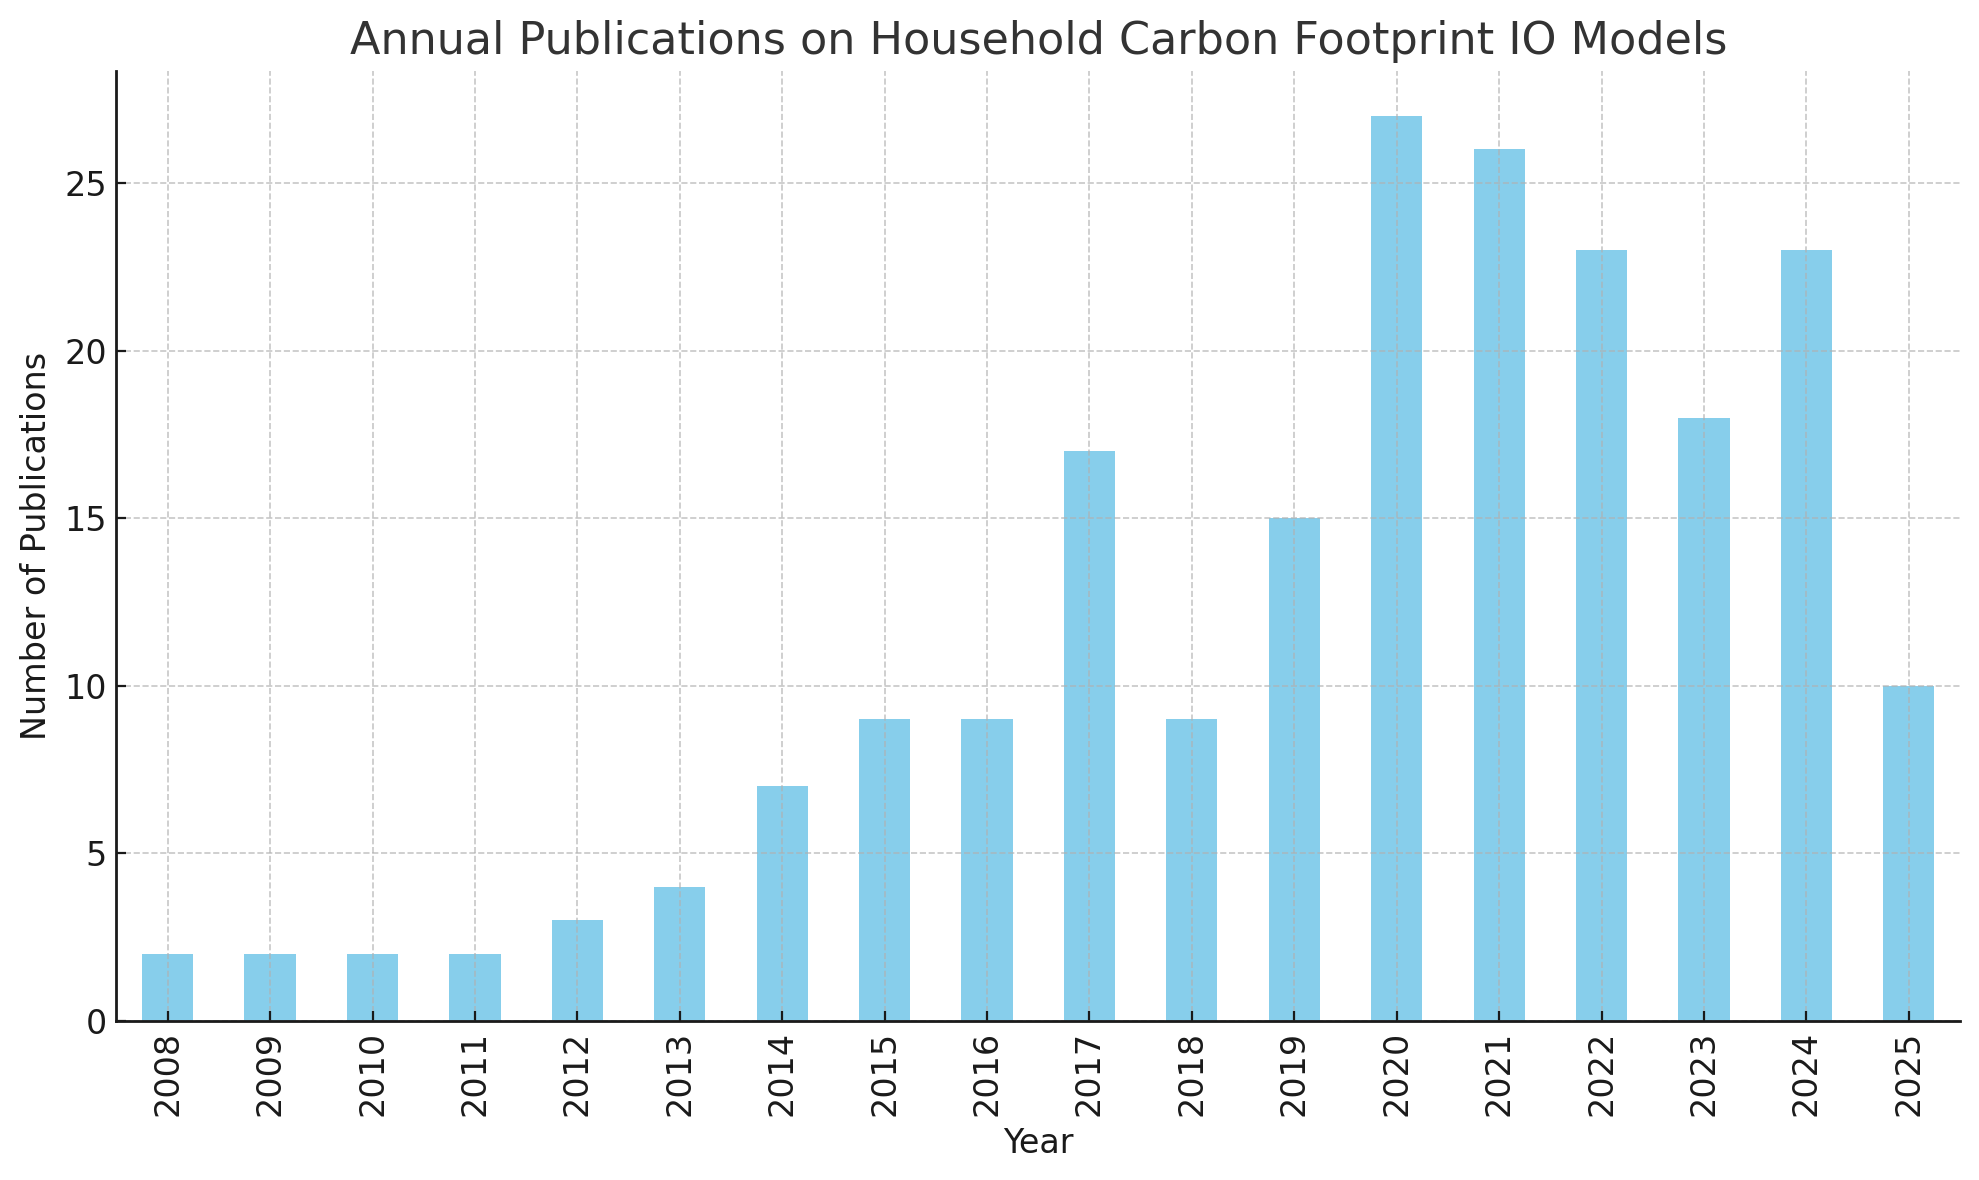
\includegraphics[width=0.7\textwidth]{Publications.png}
\caption{Annual publications on household carbon footprint using input-output models (2008--2025)}
\label{fig:Publications}
\end{figure}

\subsubsection{Lead Author Contributions}

The analysis of lead authorship indicates that a small number of researchers have contributed repeatedly as lead authors in this field (Table~\ref{tab:lead_authors}). 

\begin{table}[h]
\centering
\caption{Top lead authors, number of publications, and affiliations.}
\label{tab:lead_authors_affiliations}
\begin{tabular}{@{}lrl@{}}
\hline
\textbf{Lead Author} & \textbf{Publications} & \textbf{Affiliation} \\
\hline
Long Y. & 9 & Beijing Institute of Technology, China \\
Shigetomi Y. & 5 & Kyushu University, Japan \\
Ivanova D. & 4 & Norwegian University of Science and Technology, Norway \\
Ala-Mantila S. & 4 & Aalto University, Finland \\
Druckman A. & 3 & University of Surrey, UK \\
Liu X. & 3 & Chinese Academy of Sciences, China \\
Owen A. & 2 & University of Leeds, UK \\
Zhong H. & 2 & Chinese Academy of Sciences, China \\
Chen G. & 2 & Norwegian University of Science and Technology, Norway \\
Christis M. & 2 & University of Antwerp, Belgium \\
\hline
\end{tabular}
\end{table}


\begin{figure}[h]
\centering
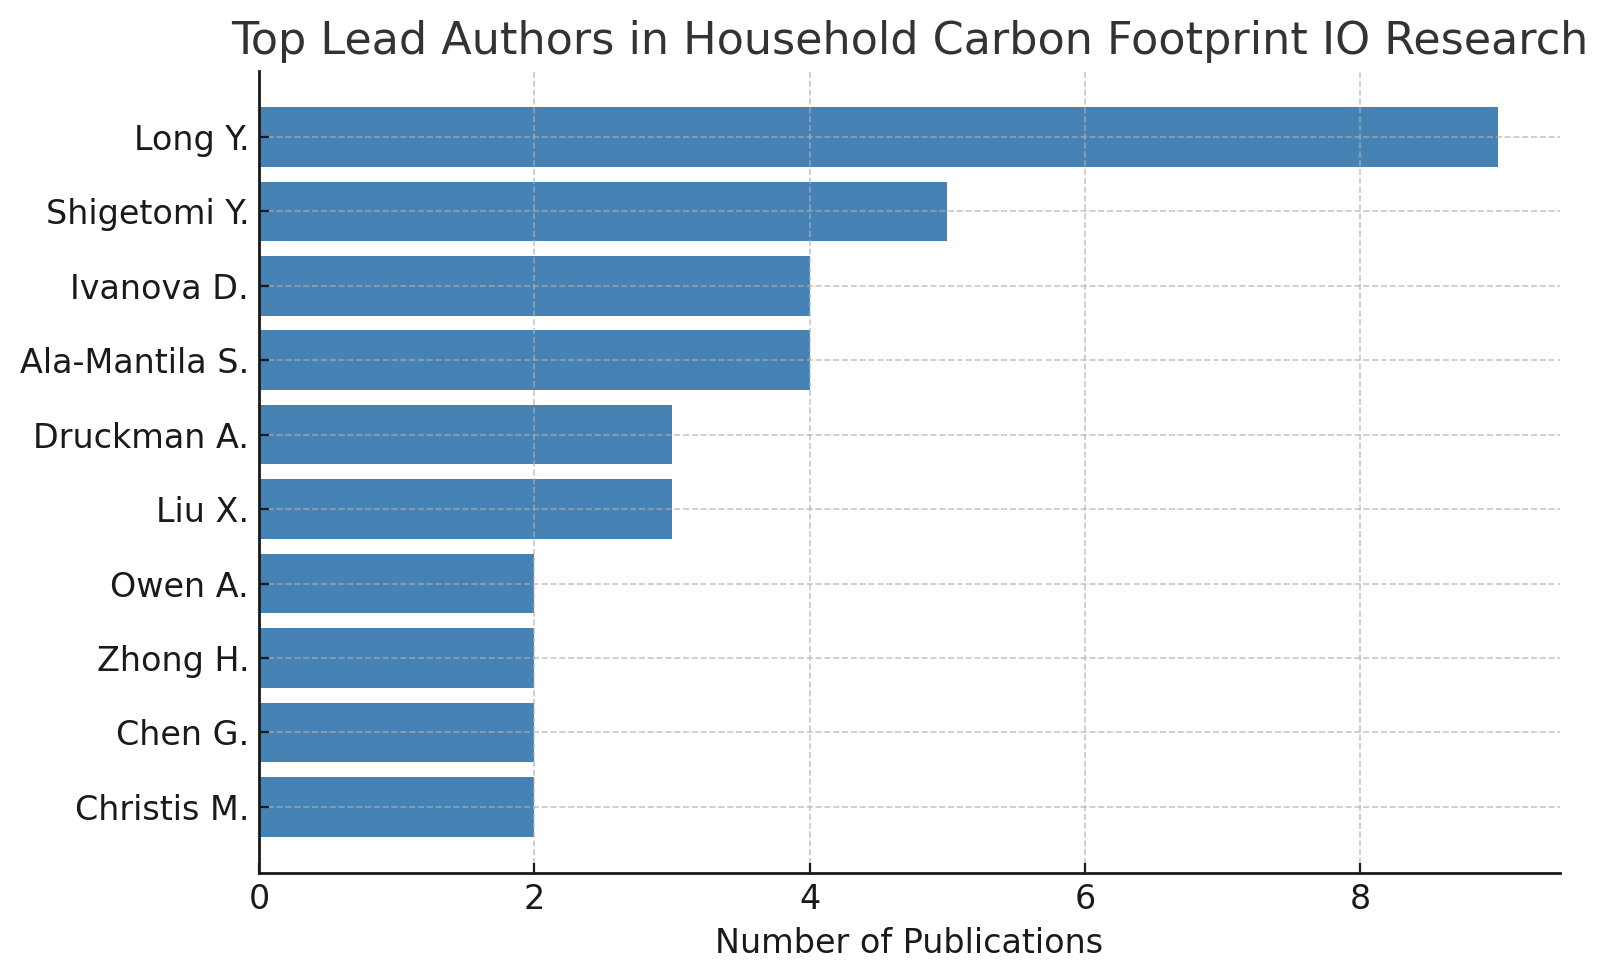
\includegraphics[width=0.7\textwidth]{Authors.png}
\caption{Top lead authors in household carbon footprint IO research}
\label{fig:lead_authors}
\end{figure}

\subsubsection{Co-authorship Patterns}

The distribution of co-authorship (Figure~\ref{fig:coauthorship}) demonstrates the collaborative nature of the field, with most publications involving multiple authors.

\begin{figure}[h]
\centering
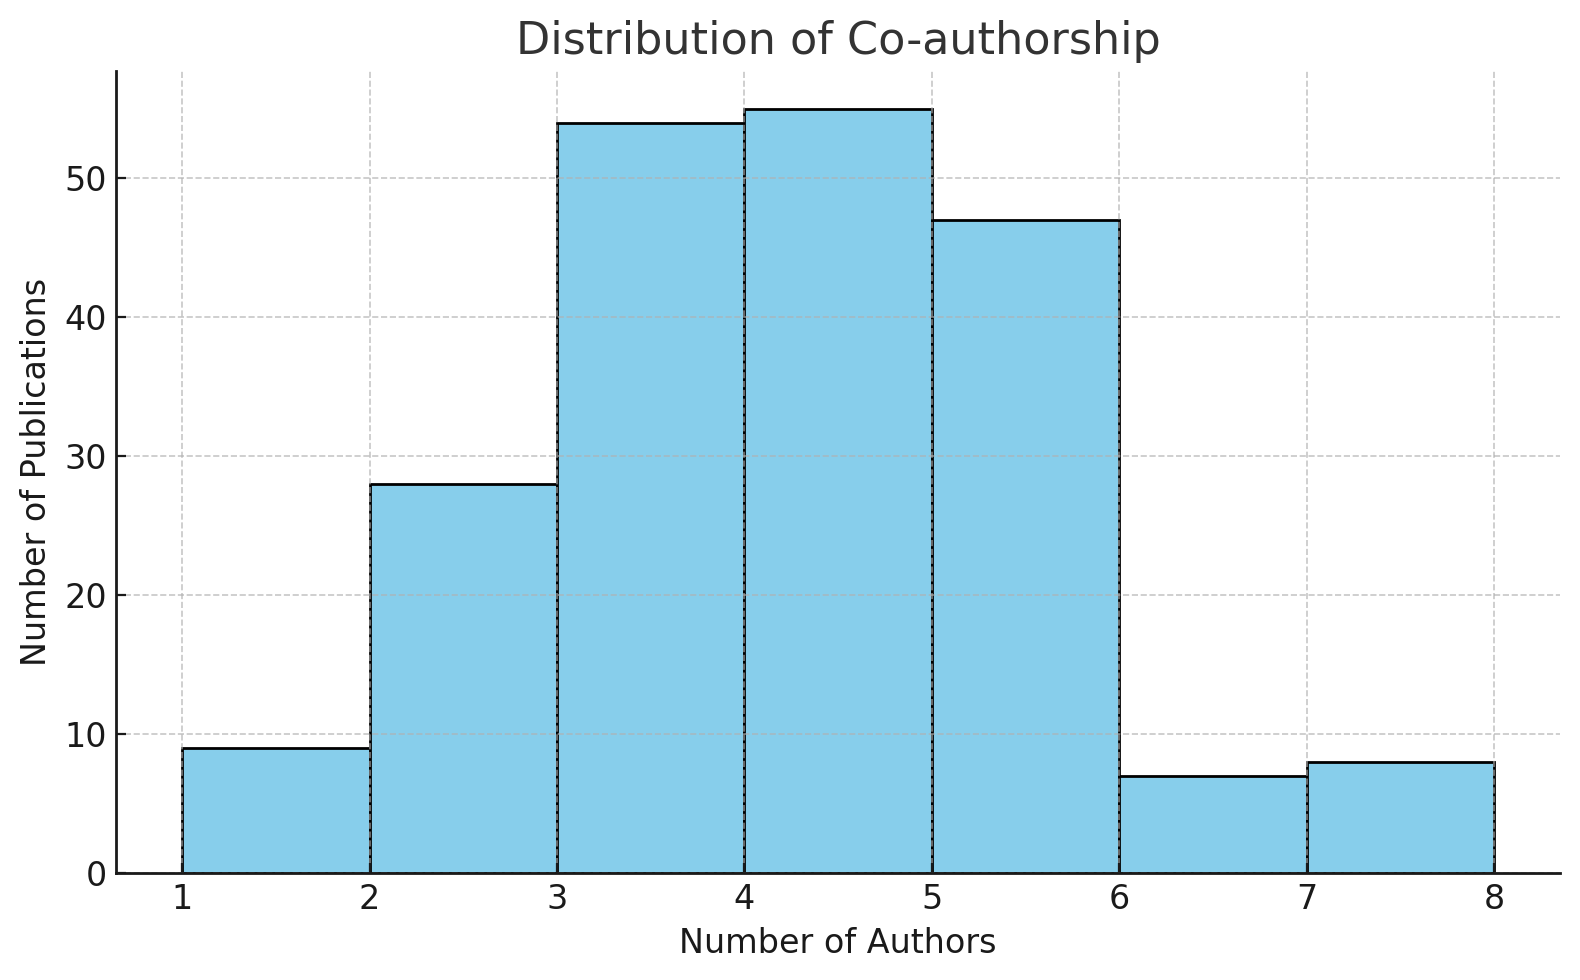
\includegraphics[width=0.7\textwidth]{Coauthors.png}
\caption{Distribution of co-authorship in household carbon footprint IO publications}
\label{fig:coauthorship}
\end{figure}

\subsubsection{Top Source Journals}

Table~\ref{tab:journal_countries} presents the top journals in terms of publication count, along with their publishing countries. The results highlight a strong presence of journals published in the Netherlands (Elsevier) and the USA.

\begin{table}[h]
\centering
\caption{Top Source Journals, Number of Publications, and Publishing Countries}
\label{tab:journal_countries}
\begin{tabular}{lll}
\hline
\textbf{Journal} & \textbf{Publications} & \textbf{Country} \\
\hline
Journal of Cleaner Production & 24 & UK / Netherlands \\
Ecological Economics & 16 & Netherlands \\
Environmental Research Letters & 14 & UK \\
Journal of Industrial Ecology & 11 & USA \\
Resources, Conservation and Recycling & 11 & Netherlands \\
Science of the Total Environment & 11 & Netherlands \\
Energy Policy & 9 & Netherlands \\
Sustainability (Switzerland) & 8 & Switzerland \\
Journal of Environmental Management & 8 & Netherlands \\
Environmental Science and Technology & 5 & USA \\
\hline
\end{tabular}
\end{table}

\subsection{Discussion}

The analysis reveals the significant growth of input-output based household carbon footprint studies, particularly after 2010. A small group of researchers, such as Long Y. and Shigetomi Y., have been especially productive. The field shows a strong collaborative character, as evidenced by the prevalence of multi-authored publications. The majority of research outputs are concentrated in leading journals published in the Netherlands, the USA, and the UK, reflecting the central role of these countries in disseminating knowledge on this topic.


\end{document}

